\documentclass{beamer}

% TODO:
% - Ajouter les timings sur le snippets
% - Disclaimer: line diff plot

\usepackage[utf8]{inputenc}
\usepackage[frenchb]{babel}
\usepackage{verbatim}
\usepackage{graphicx}
\usepackage{color}
\usepackage{hyperref}
\usepackage{verbatim}
\usepackage{url}
\usepackage{auto-pst-pdf}
\usepackage{pst-plot}
\usepackage{moreverb}
\usepackage{fancyvrb}
\usepackage{minted}
\usepackage{algpseudocode}
\usepackage{natbib}

\hypersetup{colorlinks=true, linkcolor=black, urlcolor=blue}
\usetheme{boxes}
\beamertemplatenavigationsymbolsempty
\setbeamertemplate{sections/subsections in toc}[circle]
\setbeamertemplate{footline}[frame number]
\setbeamertemplate{itemize items}[circle]
\setbeamertemplate{itemize subitem}[square]

\title{Accelerating Random Forests in Scikit-Learn}
\author{Gilles Louppe}
\institute{Université de Liège, Belgium}
\date{August 29, 2014}

\newcommand{\todo}[1]{\textcolor{red}{[TODO] #1}}

\definecolor{lightgreen}{rgb}{0.0,0.8,0.0}
\definecolor{lightblue}{rgb}{0.3,0.8,1.0}
\definecolor{lightred}{rgb}{0.874,0.180,0.105}
\definecolor{gray}{rgb}{0.4,0.4,0.4}
\definecolor{lightgray}{rgb}{0.8,0.8,0.8}
\definecolor{shadecolor}{rgb}{0.9,0.9,0.9}
\newrgbcolor{mygreen}{.00 .5 .00}
\newrgbcolor{myyellow}{.6 .6 .00}

\DeclareMathOperator*{\argmax}{arg\,max}

\begin{document}

\begin{frame}
\titlepage
\end{frame}


% Motivation ==================================================================

\begin{frame}{Motivation}

\vspace{-0.5cm}
\begin{figure}
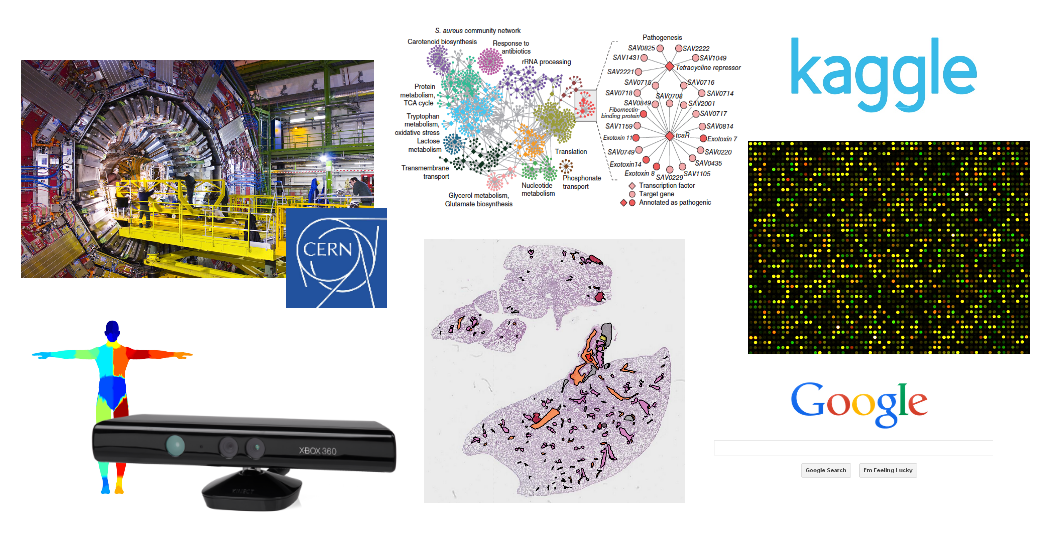
\includegraphics[scale=0.4]{./figures/motivation.png}
\end{figure}

\vspace{-0.5cm}
\begin{figure}
... and many more applications! \\
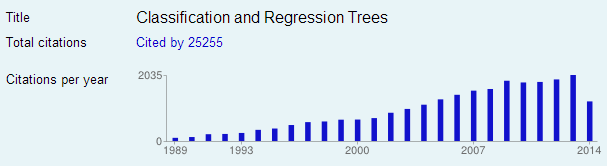
\includegraphics[scale=0.4]{./figures/cart-citations.png}
\end{figure}

%
% tree-based models are accurate models
% thousands of successful applications
%   - in vision (kinect)
%   - watson
%   - in kaggle challenges
%   - in genetics
%   - at cern
%   - and thousands of others
% not only they give good accuracy, they can also be used to better understand data (e.g. var imp)
\end{frame}


% About =======================================================================

\begin{frame}{About}


\begin{columns}
\begin{column}[t]{0.7\textwidth}
\begin{block}{Scikit-Learn}
\begin{itemize}
    \item {\bf Machine learning} library for Python
    \item Classical and {\bf well-established algorithms}
    \item Emphasis on {\bf code quality} and {\bf usability}
\end{itemize}
\end{block}
\begin{block}{Myself}
    \begin{itemize}
      \item \href{https://twitter.com/glouppe}{@glouppe}
      \item PhD student (Liège, Belgium)
      \item Core developer on Scikit-Learn since 2011\\
        \textit{Chief tree hugger}
    \end{itemize}
\end{block}
\end{column}
\begin{column}[t]{0.3\textwidth}
    \begin{figure}
    
\includegraphics[scale=0.4]{./figures/scikit-learn-logo.pdf}
    \end{figure}
\end{column}
\end{columns}

% description
% emphasis on ...
% some stats
% me = core dev of scikit-learn (as part of my thesis), author of the tree & ensemble modules
\end{frame}


% Outline =====================================================================

\AtBeginSection[]
{
\begin{frame}
  \frametitle{Outline}
  \tableofcontents[currentsection]
  % Die Option [pausesections]
\end{frame}
}

% ML 101 ======================================================================
\section{Basics}

\begin{frame}{Machine Learning 101}
  \begin{itemize}
  \item Data comes as...
    \begin{itemize}
        \vspace{0.2cm}
        \item A set of {\bf samples} ${\cal L} = \{(\mathbf{x}_i, y_i) | i = 0, \dots, N-1 \}$, with
        \vspace{0.2cm}
        \item {\bf Feature vector} $\mathbf{x} \in \mathbb{R}^p$ (= input), and
        \vspace{0.2cm}
        \item {\bf Response} $y \in \mathbb{R}$ (regression) or $y \in \{0, 1\}$ (classification) (= output)
    \end{itemize}
  \vspace{0.5cm}
  \item Goal is to...
    \begin{itemize}
        \vspace{0.2cm}
        \item Find a function $\hat{y} = \varphi(\mathbf{x})$
        \vspace{0.2cm}
        \item Such that error $L(y, \hat{y})$ on new (unseen) $\mathbf{x}$ is minimal
        \vspace{0.5cm}
    \end{itemize}
  \end{itemize}
\end{frame}


% RF ==========================================================================

\begin{frame}{Decision Trees}

\vspace{-1cm}
\begin{figure}
    \hspace*{0.5cm}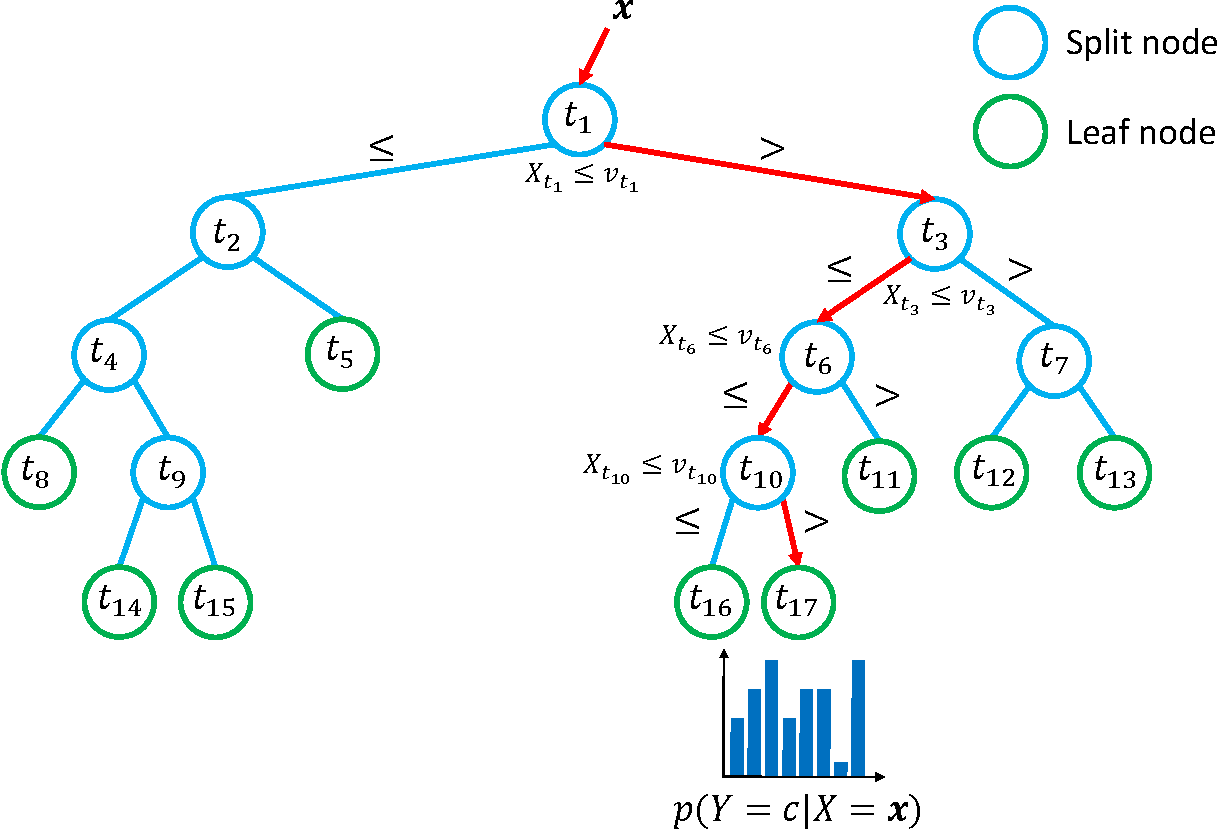
\includegraphics[scale=0.5]{./figures/tree.pdf}
\end{figure}

\vspace{-1.75cm}
$t \in \varphi$: nodes of the tree $\varphi$\\
$X_t$: split variable at $t$ \\
$v_t \in \mathbb{R}$: split threshold at $t$\\
$\varphi(\mathbf{x}) = \argmax_{c \in {\cal Y}} p(Y = c | X = \mathbf{x})$

%   - Brief description
%   - piece-wise constant approximation
%       tree vs plot
\end{frame}

\begin{frame}{Random Forests}
\begin{figure}
    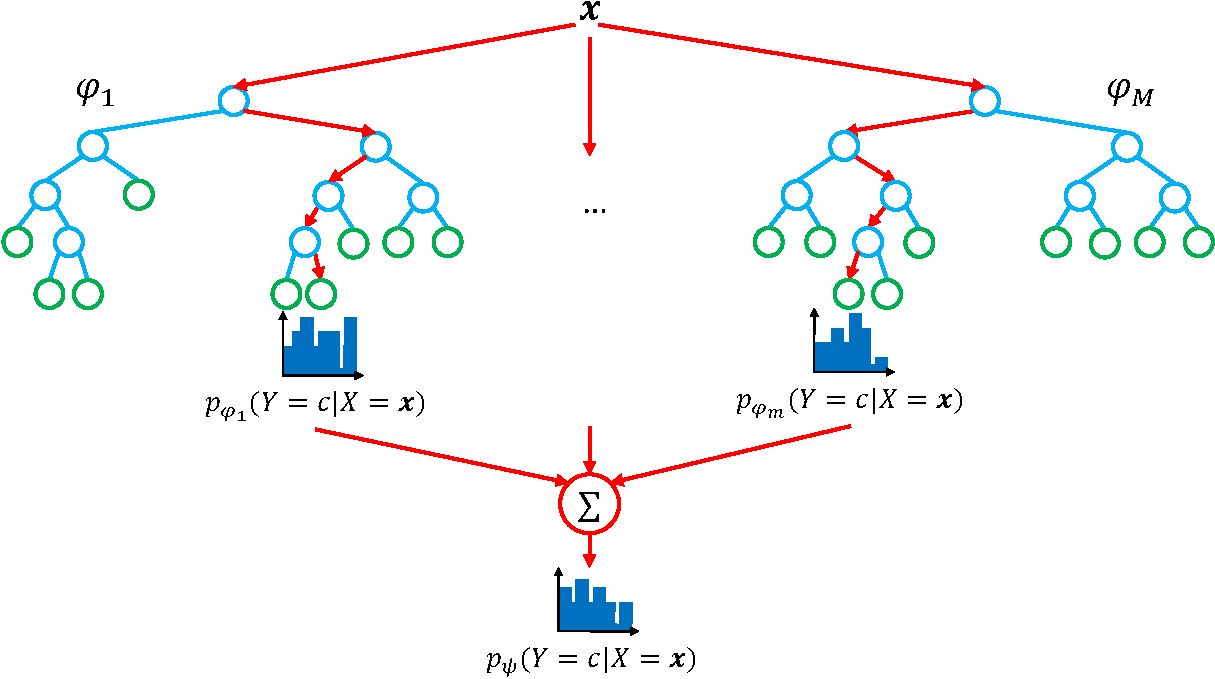
\includegraphics[scale=0.5]{./figures/forest.pdf}
\end{figure}

Ensemble of $M$ randomized decision trees $\varphi_m$\\
$\psi(\mathbf{x}) = \argmax_{c \in {\cal Y}} \frac{1}{M} \sum_{m=1}^M p_{\varphi_m}(Y = c | X = \mathbf{x})$

%   - Brief description (2d visualisation?)
\end{frame}

\begin{frame}[fragile]{Learning from data}

\begin{algorithmic}
\Function{BuildDecisionTree}{${\cal L}$}
    \State Create node $t$
    \If{the stopping criterion is met for $t$}
        \State $\widehat{y}_{t} =$ some constant value
    \Else
        \State Find the best partition ${\cal L} = {\cal L}_{L} \cup {\cal L}_{R}$
        \State $t_L = \Call{BuildDecisionTree}{{\cal L}_{L}}$
        \State $t_R = \Call{BuildDecisionTree}{{\cal L}_{R}}$
    \EndIf
    \State \Return $t$
\EndFunction
\end{algorithmic}

\end{frame}

% Timeline ====================================================================

\section{Scikit-Learn implementation}

\begin{frame}[t,fragile]{History}
%   - iterative process to figure out an efficient and flexible impl
%   - direct translation to code (in pure python) was satisfying
%   - Team effort
%       - me
%       - pprett
%       - lars
%       - ajoly
%   - Motivé par la concurrence

\begin{figure}
{\small \it Time for building a Random Forest (relative to version \texttt{0.10})}\\[1ex]
  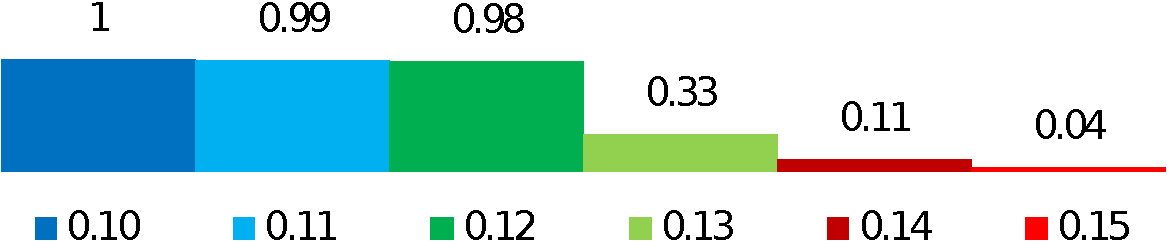
\includegraphics[scale=0.5]{./figures/fit-time.pdf}
\end{figure}

\only<+>{\texttt{0.10}: January 2012\\
\begin{itemize}
\item First sketch at \texttt{sklearn.tree} and \texttt{sklearn.ensemble}
\item Random Forests and Extremely Randomized Trees modules
\end{itemize}

\includegraphics[scale=0.5]{./figures/avatars/bholt.jpg}\quad

\includegraphics[scale=0.5]{./figures/avatars/pprett.jpg}\quad

\includegraphics[scale=0.5]{./figures/avatars/satra.jpg}\quad

\includegraphics[scale=0.5]{./figures/avatars/glouppe.jpg}\\
}

\only<+>{\texttt{0.11}: May 2012\\
\begin{itemize}
\item Gradient Boosted Regression Trees module
\item Out-of-bag estimates in Random Forests
\end{itemize}

\includegraphics[scale=0.5]{./figures/avatars/pprett.jpg}\quad

\includegraphics[scale=0.5]{./figures/avatars/amueller.jpg}
}

\only<+>{\texttt{0.12}: October 2012\\
\begin{itemize}
\item Multi-output decision trees
\end{itemize}

\includegraphics[scale=0.5]{./figures/avatars/glouppe.jpg}
%https://twitter.com/wiseio/status/273562719460925440
}

\only<+>{\texttt{0.13}: February 2013\\
\begin{itemize}
\item Speed improvements
  \begin{itemize}
    \item Rewriting from Python to Cython
  \end{itemize}
\item Support of sample weights
\item Totally randomized trees embedding
\end{itemize}

\includegraphics[scale=0.5]{./figures/avatars/pprett.jpg}\quad

\includegraphics[scale=0.5]{./figures/avatars/glouppe.jpg}\quad

\includegraphics[scale=0.5]{./figures/avatars/ndawe.jpg}\quad

\includegraphics[scale=0.5]{./figures/avatars/amueller.jpg}\quad
}

\only<+>{\texttt{0.14}: August 2013\\
\begin{itemize}
\item Complete rewrite of \texttt{sklearn.tree}
  \begin{itemize}
    \item Refactoring
    \item Cython enhancements
  \end{itemize}
\item AdaBoost module
\end{itemize}

\includegraphics[scale=0.5]{./figures/avatars/glouppe.jpg}\quad

\includegraphics[scale=0.5]{./figures/avatars/ndawe.jpg}\quad
}

\only<+>{\texttt{0.15}: August 2014\\
\begin{itemize}
\item Further speed and memory improvements
  \begin{itemize}
    \item Better algorithms
    \item Cython enhancements
  \end{itemize}
\item Better parallelism
\item Bagging module
\end{itemize}

\includegraphics[scale=0.5]{./figures/avatars/glouppe.jpg}\quad

\includegraphics[scale=0.5]{./figures/avatars/arjoly.jpg}\quad

\includegraphics[scale=0.5]{./figures/avatars/pprett.jpg}\quad

\includegraphics[scale=0.5]{./figures/avatars/ogrisel.jpg}\quad

\includegraphics[scale=0.5]{./figures/avatars/joel.jpg}\quad

\includegraphics[scale=0.666]{./figures/avatars/lars.png}
}

\end{frame}





% Overview ====================================================================

\begin{frame}[fragile]{Implementation overview}

\begin{itemize}
\item Modular implementation, designed with a strict {\bf separation of concerns}
  \begin{itemize}
    \item Builders: for building and connecting nodes into a tree
    \item Splitters: for finding a split
    \item Criteria: for evaluating the goodness of a split
    \item Tree: dedicated data structure
  \end{itemize}
\item Efficient {\bf algorithmic formulation} [See \href{http://arxiv.org/abs/1407.7502}{Louppe, 2014}]\\
  {\bf Tips.} \textit{An efficient algorithm is better than a bad one, even if the implementation of the latter is strongly optimized.}
  \begin{itemize}
    \item Dedicated sorting procedure
    \item Efficient evaluation of consecutive splits
  \end{itemize}
\item {\bf Close to the metal}, carefully coded, implementation\\
  {\small 2300+ lines of Python, 3000+ lines of Cython, 1700+ lines of tests}

\end{itemize}

\vspace{0.1cm}

\begin{minted}[fontsize=\footnotesize]{python}
# But we kept it stupid simple for users!
clf = RandomForestClassifier()
clf.fit(X_train, y_train)
y_pred = clf.predict(X_test)
\end{minted}

\end{frame}

% Iterative dev ===============================================================

\begin{frame}{Development cycle}

\vspace{-0.5cm}
\begin{figure}
\hspace*{1.6cm}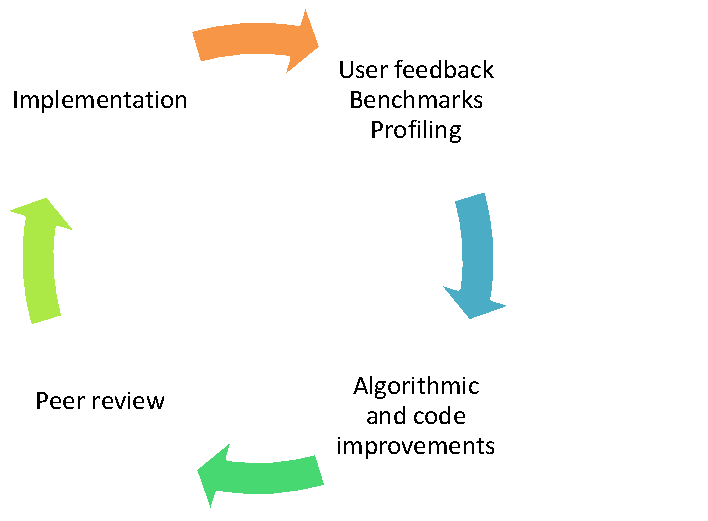
\includegraphics[scale=0.85]{./figures/iteration.pdf}
\end{figure}

% Profiling/Benchmarks <=> Algo improv or rewriting in Cython => Code review / Feedback from users ...

% You don't get it right the first time, nor the second
% but feedback from ussers, review and discussion from contributors make it converge towards an efficient solution

\end{frame}

\begin{frame}{Continuous benchmarks}
\begin{itemize}
\item During code review, changes in the tree codebase are monitored with {\bf benchmarks}.
\item {\bf Ensure performance} and code quality.
\item {\bf Avoid code complexification} if it is not worth it.
\end{itemize}

\begin{figure}

\includegraphics[scale=0.6]{./figures/bench-ogrisel.png}
\end{figure}
\end{frame}


% From Python to Cython =======================================================

\section{Python improvements}

% Ecrire l'algorithm en Cython
%   => profile & iterate
% Représentation array de l'arbre plutôt que objet
% Représentation array des données => take care of data locality and contiguity
% Parallelism

% profiling => cython plutot que python => side effects: good parallelism

% Profiling ===================================================================

\begin{frame}
\begin{center}
{\color{red} {\bf Disclaimer.} Early optimization is the root of all evil.}

\vspace{1cm}

(This took us several \textit{years} to get it right.)
\end{center}
\end{frame}

\begin{frame}[fragile]{Profiling}

Use profiling tools for {\bf identifying bottlenecks}.

\begin{minted}[fontsize=\scriptsize]{python}
In [1]: clf = DecisionTreeClassifier()

# Timer
In [2]: %timeit clf.fit(X, y)
1000 loops, best of 3: 394 mu s per loop

# memory_profiler
In [3]: %memit clf.fit(X, y)
peak memory: 48.98 MiB, increment: 0.00 MiB

# cProfile
In [4]: %prun clf.fit(X, y)
   ncalls  tottime  percall  cumtime  percall filename:lineno(function)
   390/32    0.003    0.000    0.004    0.000 _tree.pyx:1257(introsort)
     4719    0.001    0.000    0.001    0.000 _tree.pyx:1229(swap)
        8    0.001    0.000    0.006    0.001 _tree.pyx:1041(node_split)
      405    0.000    0.000    0.000    0.000 _tree.pyx:123(impurity_improvement)
        1    0.000    0.000    0.007    0.007 tree.py:93(fit)
        2    0.000    0.000    0.000    0.000 {method 'argsort' of 'numpy.ndarray' objects}
      405    0.000    0.000    0.000    0.000 _tree.pyx:294(update)
        ...
\end{minted}

% cProfile, line_profiler, memory-profiler

% benchmark on datasets
% + code profiling
% Example as
%   - Data Contiguity
%       Fortran based data (order data in the direction you'll loop over it)
%   Show call graph
\end{frame}

\begin{frame}[fragile]{Profiling (cont.)}

\begin{minted}[fontsize=\scriptsize]{python}
# line_profiler
In [5]: %lprun -f DecisionTreeClassifier.fit clf.fit(X, y)
Line     % Time     Line Contents
=================================
   ...
   256      4.5     self.tree_ = Tree(self.n_features_, self.n_classes_, self.n_outputs_)
   257
   258              # Use BestFirst if max_leaf_nodes given; use DepthFirst otherwise
   259      0.4     if max_leaf_nodes < 0:
   260      0.5         builder = DepthFirstTreeBuilder(splitter, min_samples_split,
   261      0.6                                         self.min_samples_leaf, max_depth)
   262              else:
   263                  builder = BestFirstTreeBuilder(splitter, min_samples_split,
   264                                                 self.min_samples_leaf, max_depth,
   265                                                 max_leaf_nodes)
   266
   267     22.4     builder.build(self.tree_, X, y, sample_weight)
   ...
\end{minted}

% {\footnotesize
% {\bf Cython.} Add \texttt{\#cython: profile=True} directive to enable profiling.
% }

\end{frame}

\begin{frame}[fragile]{Call graph}
\vspace{-0.65cm}

\begin{figure}
\hspace*{-1.5cm}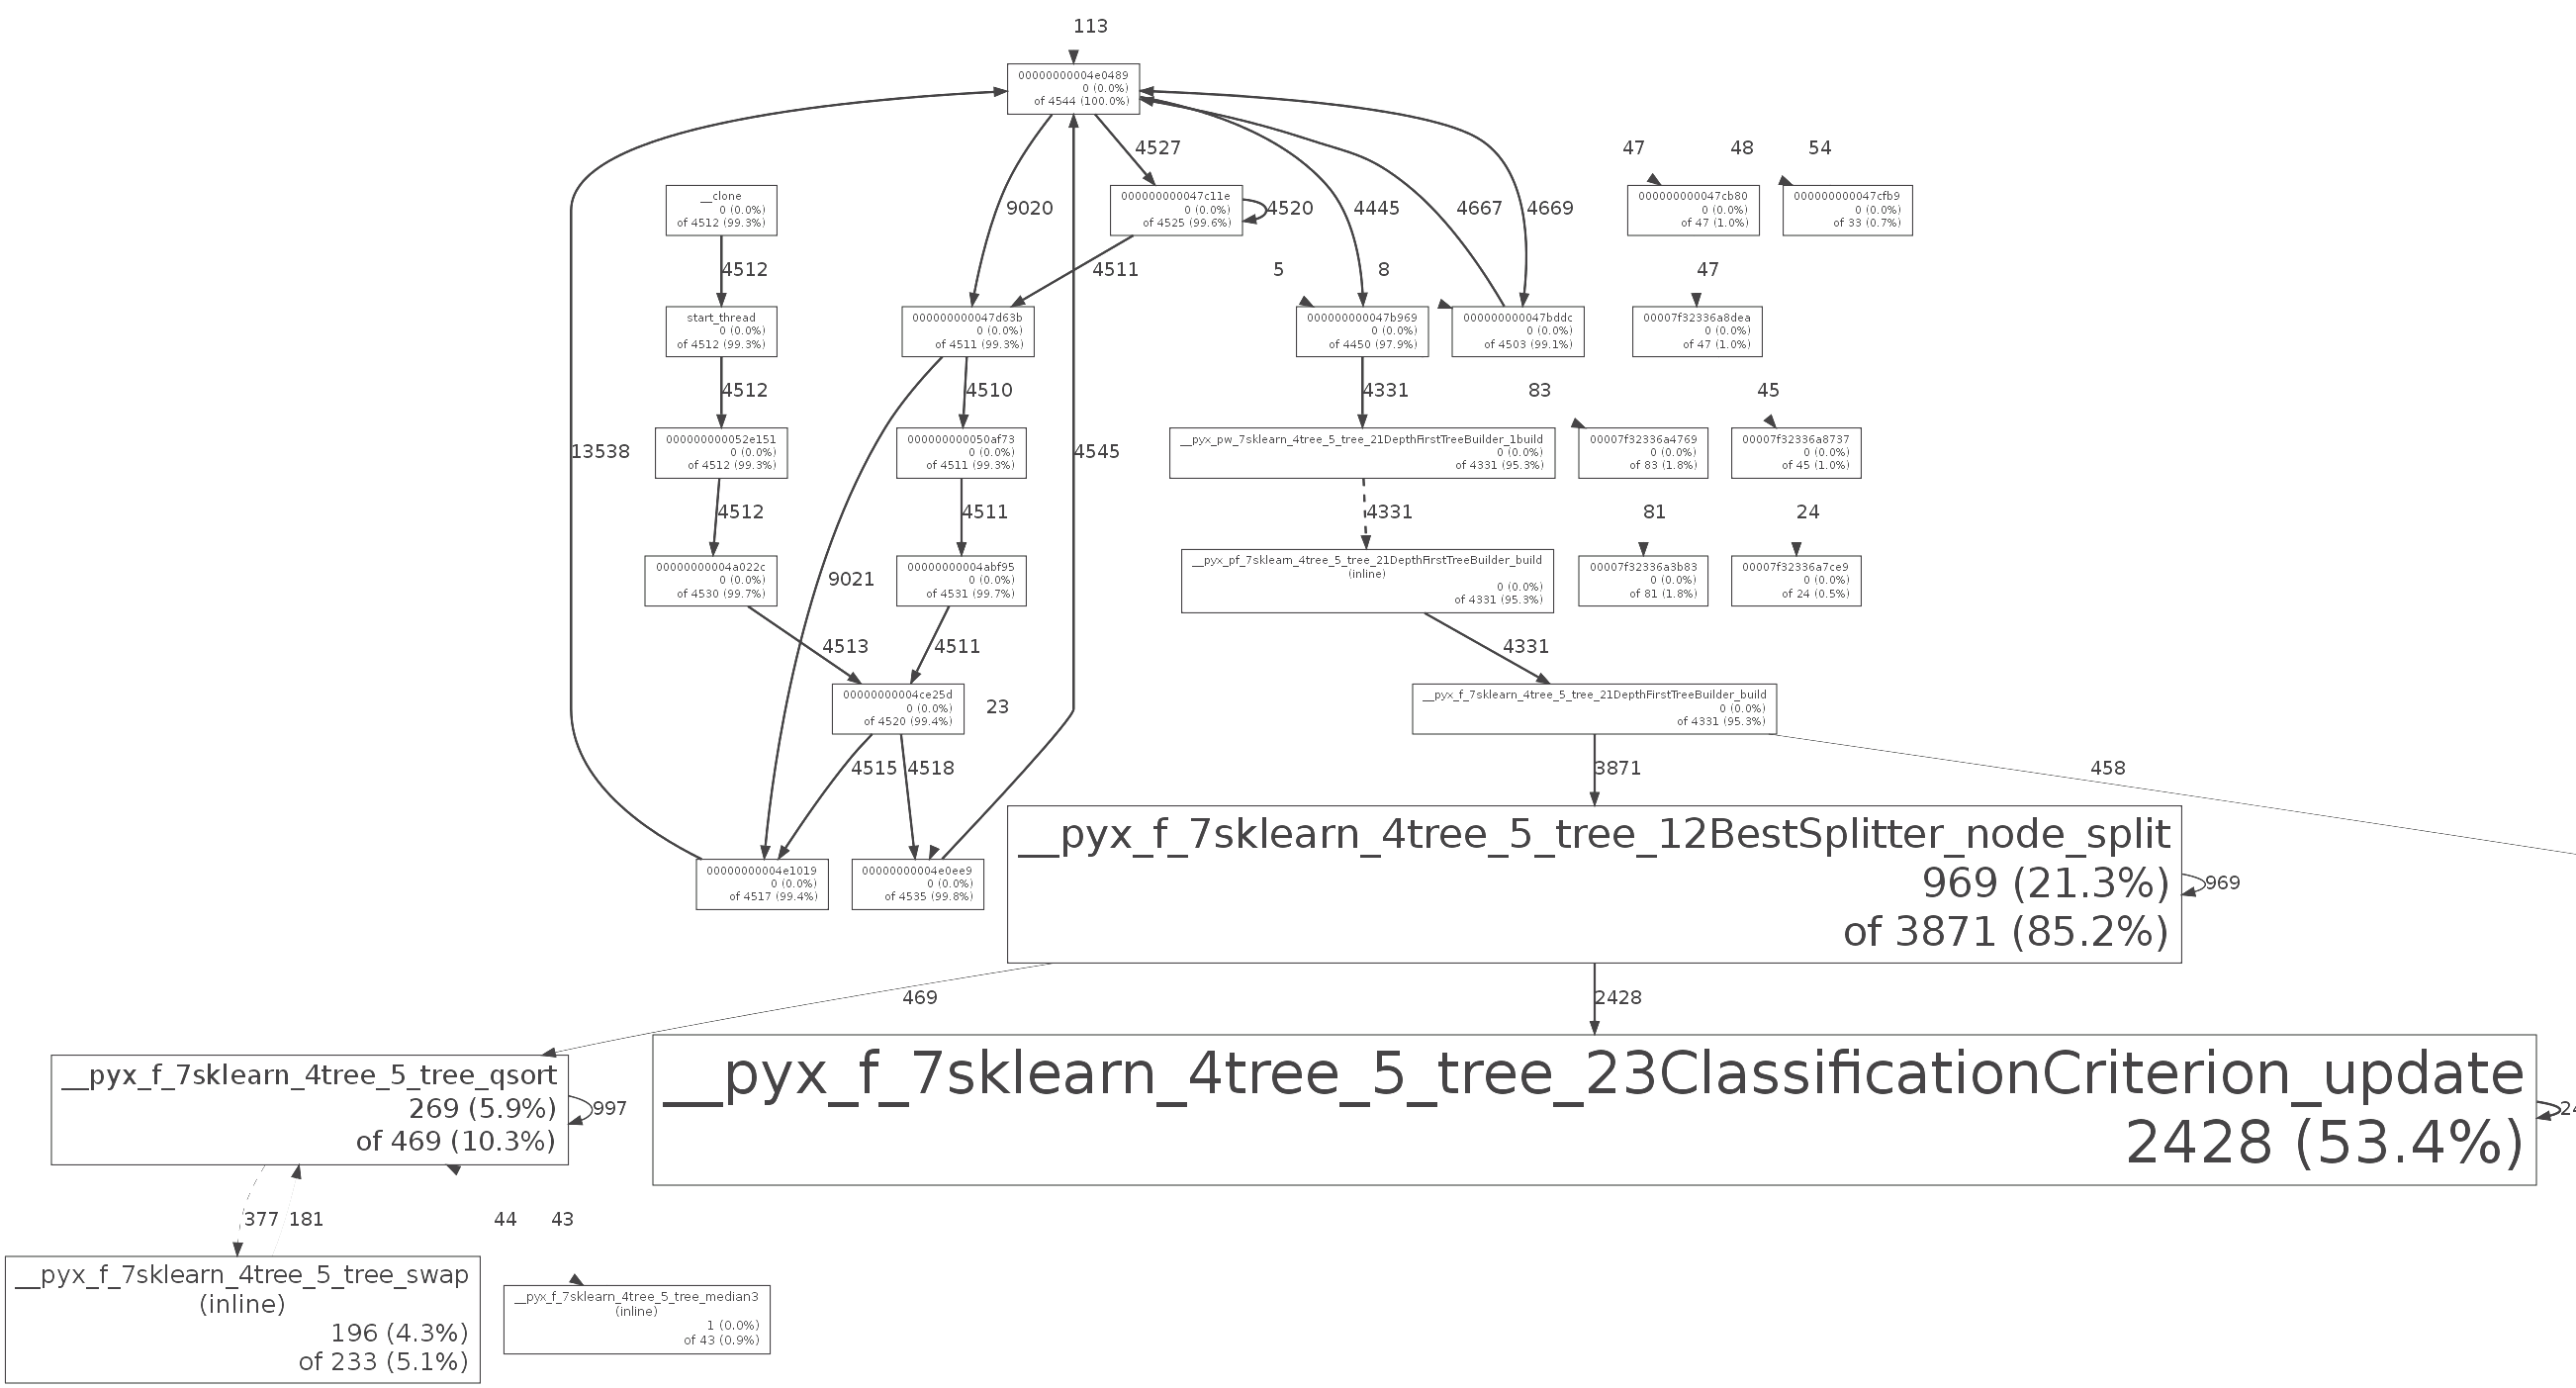
\includegraphics[scale=0.2]{./figures/graph.png}
\end{figure}

\footnotesize
\begin{verbatim}
python -m cProfile -o profile.prof script.py
gprof2dot -f pstats profile.prof -o graph.dot
\end{verbatim}

\end{frame}

\begin{frame}[fragile]{Python is slow :-(}

\begin{itemize}
\item Python overhead is {\bf too large for high-performance code}.
\item Whenever feasible, {\bf use high-level operations} (e.g., SciPy or NumPy operations on arrays)
  to {\bf limit Python calls} and rely on highly-optimized code.
\begin{minted}[fontsize=\footnotesize]{python}
def dot_python(a, b):         # Pure Python (2.09 ms)
    s = 0
    for i in range(a.shape[0]):
        s += a[i] * b[i]
    return s

np.dot(a, b)                  # NumPy (5.97 us)
\end{minted}
\item Otherwise (and only then!), {\bf write compiled C extensions} (e.g., using Cython) for critical parts.
\begin{minted}[fontsize=\footnotesize]{python}
cpdef dot_mv(double[::1] a, double[::1] b): # Cython (7.06 us)
    cdef double s = 0
    cdef int i
    for i in range(a.shape[0]):
        s += a[i] * b[i]
    return s
\end{minted}
% - cython impl
% - array rep => avoid objects
% - take care of data locality/contiguity to leverage cpu
\end{itemize}

\end{frame}

\begin{frame}[fragile]{Stay close to the metal}

%Things that worked in the case of Random Forests:

\begin{itemize}
\item Use the right data type for the right operation.
  % \begin{itemize}
  %   \item Avoid implicit (and coslty) type coercion.
  % \end{itemize}
\item Avoid repeated access (if at all) to Python objects.
  \begin{itemize}
    \item Trees are represented by single arrays.
  \end{itemize}
  {\bf Tips.} \textit{In Cython, check for hidden Python overhead. Limit yellow lines as much as possible!}\\
  \texttt{cython -a \_tree.pyx}
  \begin{figure}
  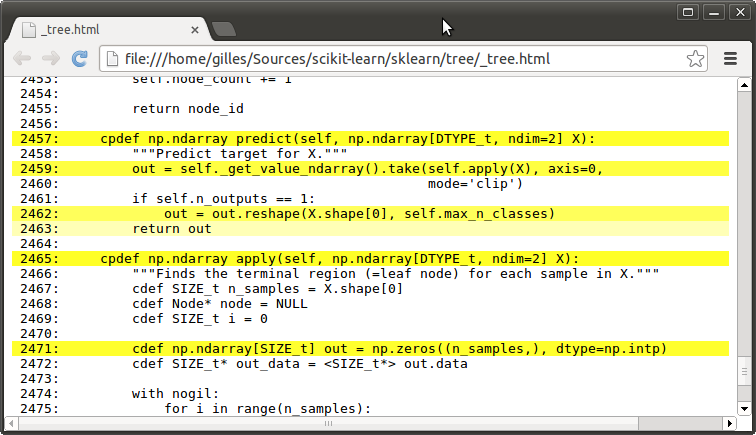
\includegraphics[scale=0.3]{./figures/cython.png}
  \end{figure}
\end{itemize}

%       array representation of the tree => faire sauter le gil
%       The current implementation is now closer to C than to Python
%       Some algorithms are naturally expressed as matrix/vactor ops. RF is not.

\end{frame}

\begin{frame}[fragile]{Stay close to the metal (cont.)}
\begin{itemize}
\item Take care of {\bf data locality and contiguity}.
  \begin{itemize}
    \item Make data contiguous to leverage CPU prefetching and cache mechanisms.
    \item Access data in the same way it is stored in memory.\\
    {\bf Tips}. \textit{If accessing values row-wise (resp. column-wise), make sure the array is C-ordered (resp. Fortran-ordered).}
\begin{minted}[fontsize=\footnotesize]{python}
cdef int[::1, :] X = np.asfortranarray(X, dtype=np.int)
cdef int i, j = 42
cdef s = 0
for i in range(...):
    s += X[i, j]  # Fast
    s += X[j, i]  # Slow
\end{minted}
    \item If not feasible, use pre-buffering.
  \end{itemize}
\end{itemize}
\end{frame}

\begin{frame}[fragile]{Stay close to the metal (cont.)}
\begin{itemize}
\item Arrays accessed with {\bf bare pointers} remain the fastest solution we have found (sadly).
  \begin{itemize}
    \item NumPy arrays or MemoryViews are slightly slower
    \item Require some {\bf \color{red} pointer kung-fu}
  \end{itemize}
\end{itemize}
  \begin{figure}
  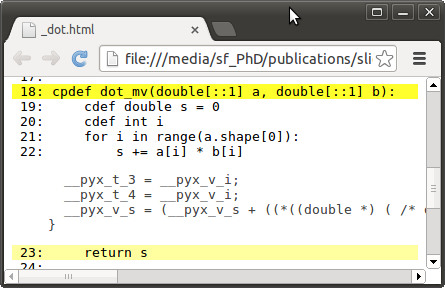
\includegraphics[scale=0.33]{./figures/1.png}\quad
  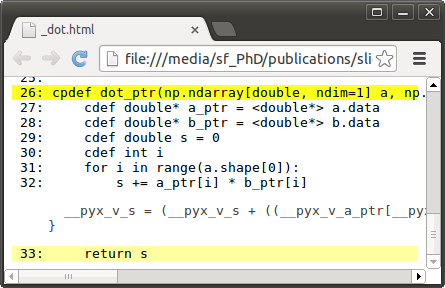
\includegraphics[scale=0.33]{./figures/2.png}\\
  \begin{minted}[fontsize=\footnotesize]{python}
            # 7.06 us                       # 6.35 us
  \end{minted}
  \end{figure}
\end{frame}

\begin{frame}{Efficient parallelism in Python is possible!}
  \begin{figure}
  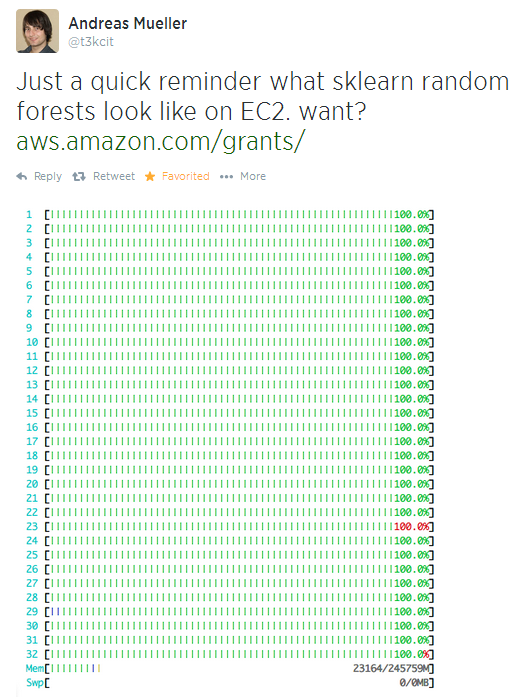
\includegraphics[scale=0.45]{./figures/parallel.png}
  \end{figure}
\end{frame}

\begin{frame}[fragile]{Joblib}
Scikit-Learn implementation of Random Forests relies on \texttt{joblib} for {\bf building trees in parallel}.
\begin{itemize}
  \item Multi-processing backend
  \item Multi-threading backend
    \begin{itemize}
      \item Require C extensions to be GIL-free \\
        {\bf Tips}. \textit{Use \texttt{nogil} declarations whenever possible.}
      \item Avoid memory dupplication
    \end{itemize}
\end{itemize}

\hspace{0.5cm}

\begin{minted}[fontsize=\footnotesize]{python}
trees = Parallel(n_jobs=self.n_jobs)(
    delayed(_parallel_build_trees)(
        tree, X, y, ...)
    for i, tree in enumerate(trees))
\end{minted}

\end{frame}


% Benchmarks ==================================================================

\begin{frame}{A winning strategy}
Scikit-Learn implementation proves to be {\bf one of the fastest} among all libraries and programming languages.
  \begin{figure}
  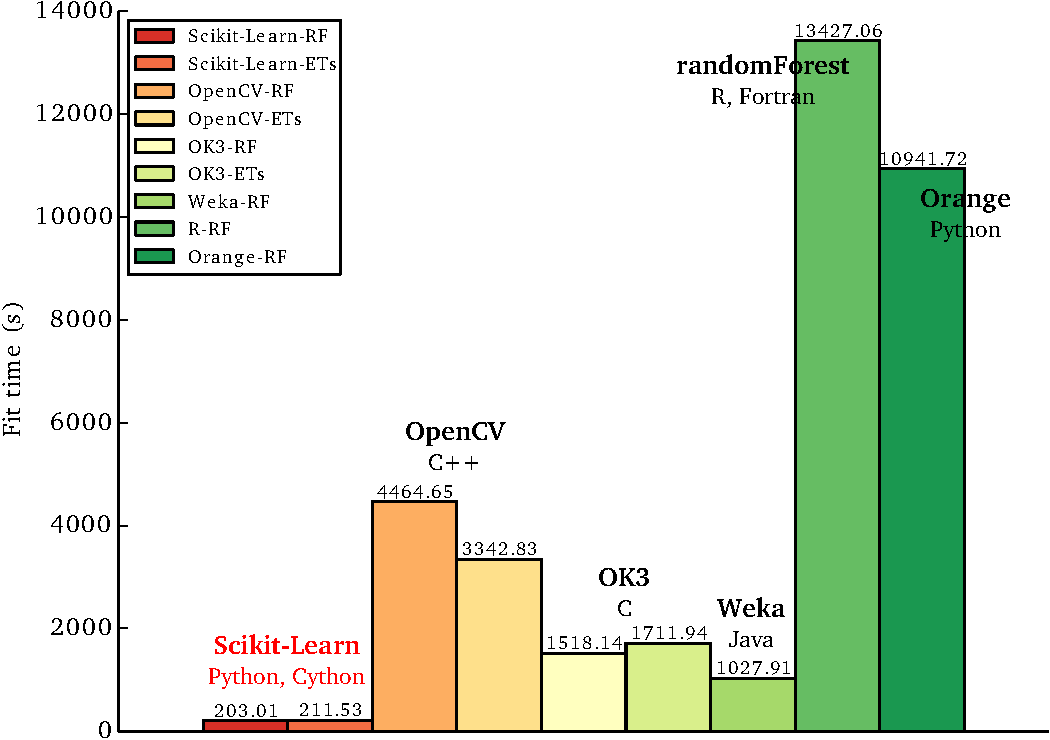
\includegraphics[scale=0.5]{./figures/bench.pdf}
  \end{figure}
\end{frame}


% Summary ====================================================================

\begin{frame}{Summary}

\begin{itemize}

\item The open source development cycle really empowered the Scikit-Learn implementation of Random Forests.

\begin{center}

\includegraphics[scale=0.5]{./figures/avatars/bholt.jpg}\quad

\includegraphics[scale=0.5]{./figures/avatars/pprett.jpg}\quad

\includegraphics[scale=0.5]{./figures/avatars/satra.jpg}\quad

\includegraphics[scale=0.5]{./figures/avatars/glouppe.jpg}\quad

\includegraphics[scale=0.5]{./figures/avatars/ndawe.jpg}\\

\includegraphics[scale=0.5]{./figures/avatars/amueller.jpg}\quad

\includegraphics[scale=0.5]{./figures/avatars/arjoly.jpg}\quad

\includegraphics[scale=0.5]{./figures/avatars/ogrisel.jpg}\quad

\includegraphics[scale=0.5]{./figures/avatars/joel.jpg}\quad

\includegraphics[scale=0.666]{./figures/avatars/lars.png}
\end{center}

\item Combine algorithmic improvements with code optimization.

\item Make use of profiling tools to identify bottlenecks.

\item Optimize only critical code!

\end{itemize}

\end{frame}

\end{document}
